% Created 2018-05-01 Tue 16:31
% Intended LaTeX compiler: pdflatex
\documentclass[final]{beamer}
	         \usetheme{ph}
           \usepackage[orientation=portrait,size=a0,scale=1.4]{beamerposter}
           \usepackage[absolute,overlay]{textpos}
	         \usepackage[authoryear]{natbib}


\setlength{\paperwidth}{36in}
\setlength{\paperheight}{48in}
\setlength{\textwidth}{0.98\paperwidth}
\setlength{\textheight}{0.98\paperheight}
\graphicspath{{../output/figures/}{../lib/}}
\usepackage[export]{adjustbox}
\usepackage{graphicx,caption}
\usepackage{minted}
\usepackage{eurosym}
\usepackage{listings}
\usepackage{textcomp}
\usepackage{bibentry}
\newcommand\sumin{\sum_{i=1}^{n}}
\newcommand{\Xoi}[1]{#1(i)}
\newcommand{\frakPQ}[2]{\frac{\Xoi{#1}}{\Xoi{#2}}}
\newcommand{\DKLPQ}[3]{D_{\mathrm{KL}}(#1 #3 #2)}
\date{}
\newcommand{\auth}{Philipp Homan, MD, PhD}
\newcommand{\authemail}{phoman1@northwell.edu}
\newcommand{\authtwitter}{@philipphoman}
\newcommand{\authgithub}{github.com/philipphoman}
\author{
Philipp Homan$^{1}$
\\
\vspace{5mm}
\normalsize{$^{1}$Department of Psychiatry,}
\normalsize{The Donald and Barbara Zucker}
\normalsize{School of Medicine at Northwell/Hofstra,}
\normalsize{Hempstead, NY}
}
\usetheme{default}
\date{2018-05-01 16:31}
\title{Using org-mode for scientific posters}
\begin{document}

\begin{frame}[fragile,label={sec:org48aedac}]{}
 \begin{columns}
\begin{column}[t]{0.45\columnwidth}
\begin{block}{Background}
\begin{itemize}
\item Here we show how org-mode (version 
9.1.9) and emacs (version 
25.1.1) can be used to make decent looking scientific
posters
\item With org-mode we can populate the poster with code, graphs and numbers
from inline code in languages such as R, python, Matlab and even shell
scripting
\item For example, this poster was created on 2018-05-01 16:31 on
Ubuntu 17.04.
\item Inline code could look like this (which will produce a graph; 
Fig. \ref{fig:orgf02b88f}):
\end{itemize}

\begin{columns}
\begin{column}[T]{0.68\columnwidth}
\begin{minted}[linenos=true,bgcolor=lightgray]{r}
set.seed(20180402)
x1 <- rnorm(100, 0, 1)
x2 <- rnorm(100, 0.5, 1)
hist(x1, col="red")
hist(x2, col="blue", add=TRUE)
\end{minted}

\begin{figure}[htbp]
\centering
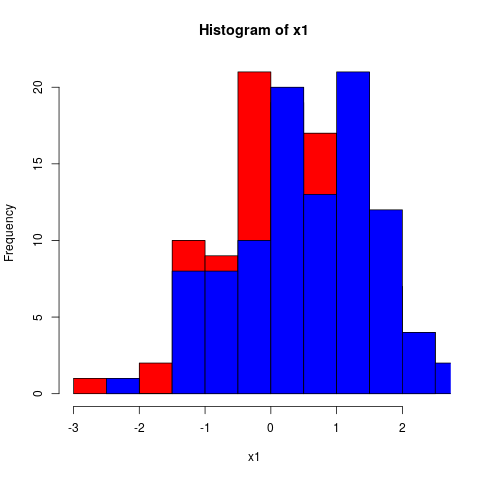
\includegraphics[width=.9\linewidth]{3.png}
\caption{\label{fig:orgf02b88f}
This is the output.}
\end{figure}
\end{column}
\end{columns}
\end{block}

\begin{block}{Inline code and tables}
\begin{itemize}
\item Tables are powerful in org-mode and even include spreadsheet
capabilities
\item Some code to process the first vector from above to make a table out
of its summary could look like this, which would result in a little
table (Table \ref{tab:orga274aaf}) :
\end{itemize}

\begin{columns}
\begin{column}[T]{0.78\columnwidth}
\begin{minted}[linenos=true,bgcolor=lightgray]{r}
library(broom)
library(dplyr)
t1 <- tidy(round(summary(x1), 2)) 
t2 <- tidy(round(summary(x2), 2))

# This will export as a table
rbind(t1, t2) %>%
mutate(name=c("x1", "x2"))
\end{minted}

\vspace{2cm}
\small
\begin{table}[htbp]
\caption{\label{tab:orga274aaf}
A table summarizing the two distributions.}
\centering
\begin{tabular}{rrrrrrl}
\hline
minimum & q1 & median & mean & q3 & maximum & name\\
\hline
-2.29 & -0.49 & 0.11 & 0.14 & 0.8 & 2.47 & x1\\
-2.17 & -0.45 & 0.07 & 0.13 & 0.85 & 2.23 & x2\\
\hline
\end{tabular}
\end{table}
\end{column}
\end{columns}
\end{block}
\end{column}

\begin{column}[t]{0.45\columnwidth}
\begin{block}{Graphics}
\begin{itemize}
\item We can use shell scripting to grab an image with curl from the
internet (Fig. \ref{fig:orgcbcb8d7}):
\end{itemize}

\begin{columns}
\begin{column}[T]{0.78\columnwidth}
\footnotesize
\begin{minted}[linenos=true,bgcolor=lightgray]{bash}
# Download emacs icon from gnu.org
curl -0 https://www.gnu.org/software/emacs/images/emacs.png
\end{minted}
\normalsize

\vspace{2cm}

\begin{figure}[htbp]
\centering

\includegraphics[page=9,width=0.2\textwidth]{emacs.png}
\caption{\label{fig:orgcbcb8d7}
This is the downloaded image.}
\end{figure}
\end{column}
\end{columns}
\end{block}

\begin{block}{Math}
\begin{itemize}
\item Let's describe how to compute the distance between the
two simulated distributions \(x1\) and \(x2\) from before:
\end{itemize}

\begin{columns}
\begin{column}[T]{0.78\columnwidth}
\small
The Kullback-Leibler (KL) divergence measures the difference between two
probability distributions (i.e., the loss of information when one
distribution is used to approximate another). The KL divergence is thus
defined as
\begin{align} 
\label{eq:KL} 
\DKLPQ{P}{Q}{\|} = \sumin \Xoi{P} \log \frakPQ{P}{Q}
\end{align} 
with \(P\) and \(Q\) being two probability distribution functions and \(n\)
the number of sample points. Since \(\DKLPQ{P}{Q}{\|}\) is not equal to
\(\DKLPQ{Q}{P}{\|}\), a symmetric variation of the KL divergence can be
derived as follows:
\small
\begin{align} 
\label{eq:KL2} 
\DKLPQ{P}{Q}{,} = \sumin \Big(\Xoi{P} \log \frakPQ{P}{Q} + \Xoi{Q} \log \frakPQ{Q}{P} \Big).
\end{align}
\end{column}
\end{columns}
\end{block}

\begin{block}{Columns}
\begin{columns}
\begin{column}[T]{0.48\columnwidth}
\captionsetup{justification=justified,width=.85\linewidth}
\begin{figure}[htbp]
\centering
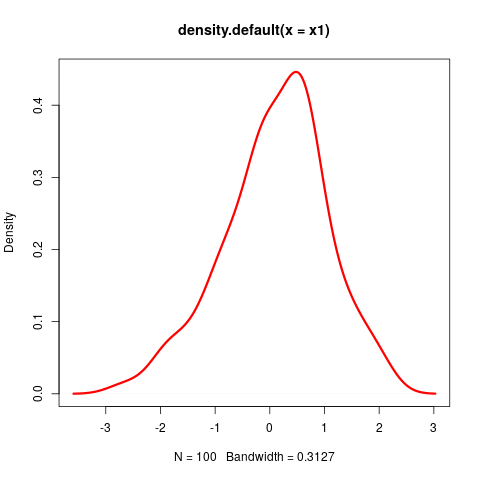
\includegraphics[width=.9\linewidth]{4l.png}
\caption{\label{fig:orgf1fb0dc}
This is the left figure of a two-column block, showing the density of \(x1\).}
\end{figure}
\end{column}

\begin{column}[T]{0.48\columnwidth}
\captionsetup{justification=justified,width=.85\linewidth}
\begin{figure}[htbp]
\centering
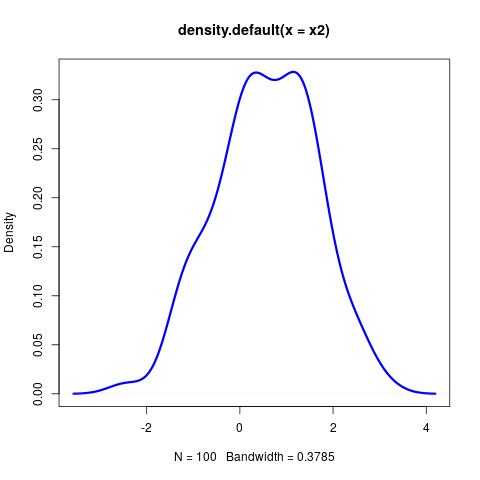
\includegraphics[width=.9\linewidth]{4r.png}
\caption{\label{fig:orgf00fe3b}
This is the right figure. It shows the density of \(x2\).}
\end{figure}
\end{column}
\end{columns}
\end{block}

\begin{block}{Conclusions}
\begin{itemize}
\item This example is meant to show how versatile org-mode is
\item Scientific posters can be produced with a simple text editor
\end{itemize}
\end{block}
\end{column}
\end{columns}
\end{frame}
\end{document}
